\documentclass{trlnotes}
\setlayout{hardcopy}
\usepackage{silence}
\WarningFilter{latex}{Reference}
\graphicspath{{../../img/}}

\begin{document}
    \paragraph{Разностный метод для общего уравнения теплопроводности, явная схема}

    \begin{de}
        Общее \ti{уравнение теплопроводности} выглядит вот так:
        \[
            \dfrac{\pd u}{\pd t} = a_0 \dfrac{\pd^2 u}{\pd x^2} + a_1 \dfrac{\pd y}{\pd x} + a_2 u + f.
        \]
        Функции $a_i$ и $f$ зависят от $x$ и $t$.
    \end{de}

    Работать будем, как всегда, на отрезке $[a, \, b]$; временной отрезок будет $[0, \, T]$.

    \begin{de}
        У уравнения теплопроводности бывает \ti{начальное условие}:
        \[
            u(x, \, 0) = \varphi(x),            
        \]
        а также три типа \ti{граничных условий}
        \begin{enumerate}
            \item $u(a, \, t) = \psi_0(t)$, $u(b, \, t) = \psi_1(t)$.
            \item $\dfrac{\pd u}{\pd x}(a, \, t) = \psi_0(t)$, $\dfrac{\pd u}{\pd x}(b, \, t) = \psi_1(t)$.
            \item $\dfrac{\pd u}{\pd x} - \alpha u \big|_{x = a} = \psi_0(t)$, $\dfrac{\pd u}{\pd x} - \beta u \big|_{x = b} = \psi_1(t)$.
        \end{enumerate}
    \end{de}
    Сетка характеризуется такими же, как обычно, величинами:
    \[
        \begin{array}{lll}
            x_i = a + ih, & h = \dfrac{b - a}{h}, & i \in 0\ldots n; \\
            t_k = k\tau, & \tau = \dfrac{T}{M}, & k \in 0 \ldots M.
        \end{array}
    \]

    Положим $u_i^k = u(x_i, \, t_k)$ и
    \[
        Lu = a_0 \dfrac{\pd^2 u}{\pd x^2} + a_1 \dfrac{\pd y}{\pd x} + a_2 u.
    \]
    Тогда
    \[
        (\tilde{L}u)_i^k = a_0 \dfrac{u_{i+1}^k - 2u_i^k + u_{i - 1}^k}{h^2} + a_1 \dfrac{u_{i + 1}^k - u_{i - 1}^k}{2h} + a_2 u_i^k.
    \]
    Есть два варианта для производной по времени:
    \begin{align*}
        &\text{A:} \quad \dfrac{\pd u}{\pd t}(x_i, \, t_k) \approx \dfrac{u^{k + 1}_i - u^k_i}{\tau}, \\
        &\text{B:} \quad \dfrac{\pd u}{\pd t}(x_i, \, t_k) \approx \dfrac{u^{k}_i - u^{k-1}_i}{\tau}.
    \end{align*}
    Для варианта A получается 
    \[
        \boxed{\dfrac{u_i^{k + 1} - u_i^k}{\tau} = \tilde{L}u_i^k + f(x_i, \, t_k)}\,.
    \]
    Это простейшая явная схема. 

    \begin{figure}[h] \label{fig:therm-simple}
        \begin{center}
%             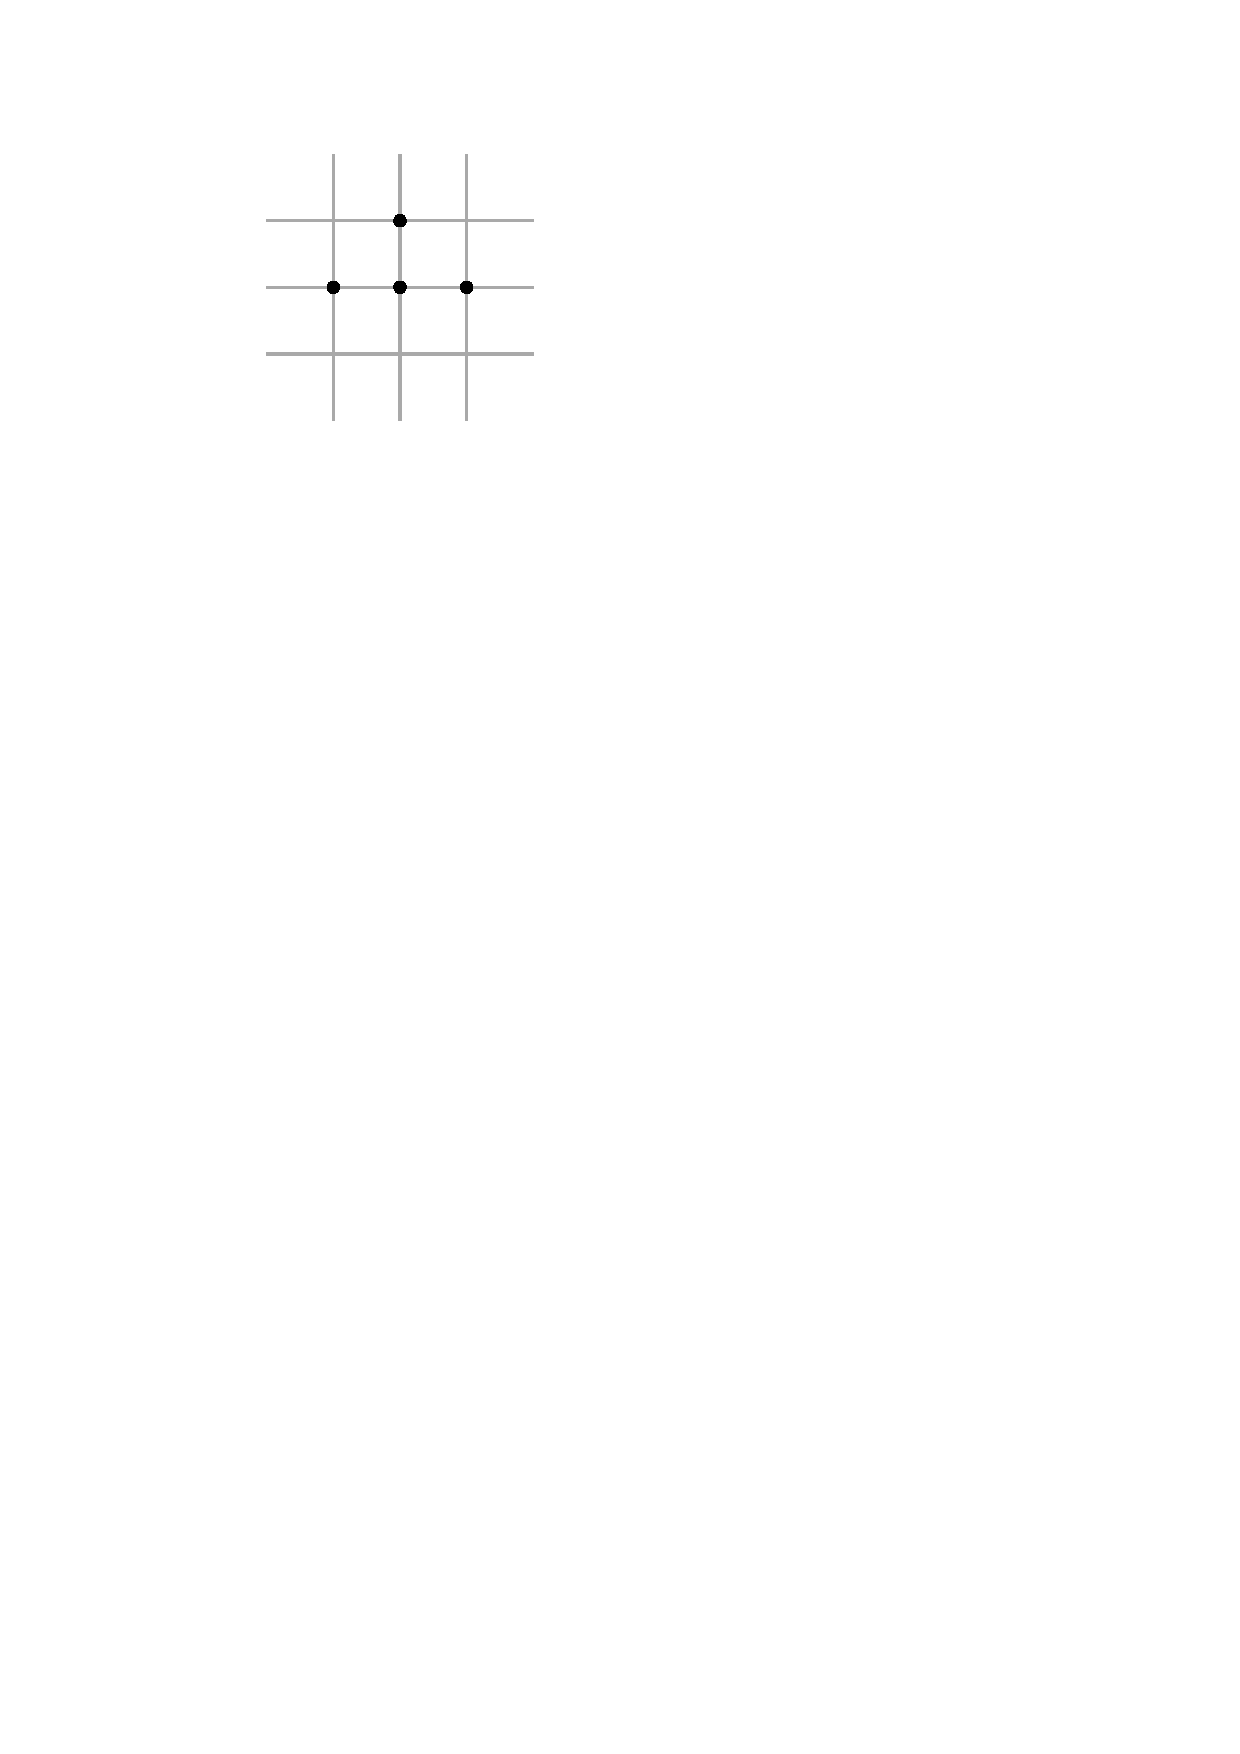
\includegraphics[scale=0.9]{../img/therm-simple.pdf}
          забыли
        \end{center}
        \caption{Простейшая явная схема для уравнения теплопроводности.}
    \end{figure}

    В таком виде уравнения можно писать для $i \in 1\ldots n-1$, $k\in 0\ldots M-1$; нужны дополнительные с граничными условиями. 

    \begin{itemize}
        \item Начальные условия: $u_i^0 = \varphi(x_i)$.
        \item Граничные условия:
        \begin{enumerate}
            \item $u_0^k = \alpha_1(t_k)$, $u_n^k = \alpha_2(t_k)$; при этом выполняются условия согласования \ti{нулевого порядка}
            \[
                \varphi(a) = \alpha_1(0), \quad \varphi(b) = \alpha_2(0).
            \]
            \item Для типов II, III используются такие же трюки, как в обычных диффурах. Надо аппроксимировать производные. Можно применять метод фиктивных точек или метод исключения главного члена погрешности.

            В угловых точках снова возникнет два разных условия:
            \[
                u_0^0 = \varphi(a) \text{ и } \dfrac{\pd u}{\pd x}(a, \, 0) = \beta_1(0) u_0^0 + \alpha_1(0).
            \]
            Будет ли выполняться равенство
            \[
                \varphi'(a) = \beta_1(0) u_0^0 + \alpha_1(0)?
            \]
            Оно называется \ti{условием согласования I порядка}. Без него уравнения не станут формально противоречивы.
        \end{enumerate}
    \end{itemize}

    Если разрешить уравнения относительно $u_i^{k + 1}$, получится 
    \[
        u_{i}^{k + 1} = A_i^k u_{i-1}^k + B_i^k u_i^k + C_i^k u_{i+1}^k + D_i^k.
    \]
    Коэффициенты выражаются по формулам
    \[
        \begin{array}{ll}
            A_i^k = \sigma a_0 - \sigma a_1 \dfrac{h}{2}, & C_i^k = \sigma a_0 + \sigma \dfrac{h}{2} a_1, \\
            B_i^k = 1 - 2 \sigma a_0 + \tau a_2,  &D_i^k = \tau f(x_i, \, t_k),
        \end{array}
    \]
    где $\sigma = \dfrac{\tau}{h^2}$.

    Можно просто двигаться вперёд по \ti{слоям}~--- множествам точек с постоянным временем; значения находятся последовательно.
\end{document}
